\section{Caso de estudio}
Para el actual proyecto se necesita un groupware al cu\'al se le pueda acoplar la arquitectura para poder analizar sus datos, en este caso el sistema seleccionado es un videojuego colaborativo de disparos en primera persona: \textit{AssaultCube}. Este groupware en particular tiene las caracter\'isticas de ser distribuido y s\'incrono seg\'un la clasificaci\'on de Ellis\cite{ellis1991groupware}, contiene varios tipos de elementos y los modos multijugador son entre equipos en los cuales se requiere de una buena colaboraci\'on para cumplir los objetivos de la actividad. 

\begin{figure}[h!]
\centering
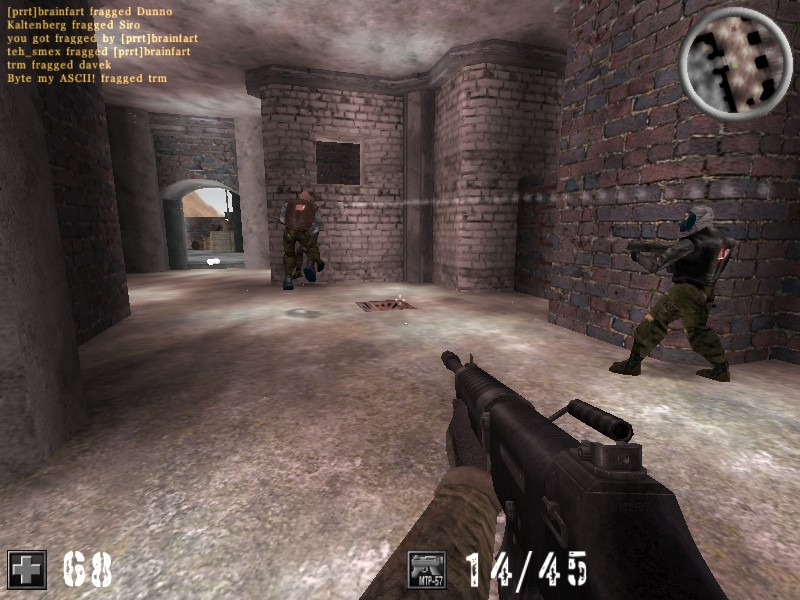
\includegraphics[scale=.15]{images/assaultcube}
\caption{Assault Cube}
\label{gw:asscb}
\end{figure}

En la Tabla 1 se muestran las interacciones identificadas en el juego, en ellas se encuentran algunos elementos del modelo como pueden ser Actores, Tareas y Objetos,  esto nos da la pauta para empeazar a dise\~nar nuestro modelo. 

\definecolor{LightCyan}{rgb}{0.29,0.67,0.77}
\begin{center}
\label{AC:interacciones}
\begin{longtable}{|p{5cm}|p{7cm}|}

\caption{Tabla de interacciones detectadas en \textit{Assault Cube}}\\
\hline
\rowcolor{LightCyan}\textbf{Interacci\'on} & \textbf{Elementos identificados}\\
\hline
\endfirsthead
\multicolumn{2}{c}%
{\tablename\ \thetable\ -- \textit{... Contin\'ua de p\'agina anterior}} \\
\hline
\textbf{Interacci\'on} & \textbf{Elementos identificados} \\
\hline
\endhead
\hline \multicolumn{2}{r}{\textit{Contin\'ua en siguiente p\'agina...}} \\
\endfoot
\hline
\endlastfoot
\textbf{Jugador se Mueve} & Actor: Jugador; Tarea: Moverse\\\hline

\textbf{Jugador salta} & Actor: Jugador; Tarea: Saltar\\\hline

\textbf{Jugador dispara arma} & Actor: Jugador; Tarea: Saltar; Objeto: Arma\\\hline

\textbf{Jugador recarga arma} & Actor: Jugador; Tarea: Recargar; Objeto: Arma\\\hline

\textbf{Jugador dispara arma} & Actor: Jugador; Tarea: Saltar; Objeto: Arma\\\hline

\textbf{Jugador cambia arma} & Actor: Jugador; Tarea: Cambiar; Objeto: Arma\\\hline

\textbf{Jugador obtiene mejora de salud} & Actor: Jugador; Tarea: Obtener; Objeto: Mejora de salud\\\hline

\textbf{Jugador obtiene protecci\'on} & Actor: Jugador; Tarea: Obtener; Objeto: Protecci\'on\\\hline

\textbf{Jugador obtiene munici\'on} & Actor: Jugador; Tarea: Obtener; Objeto: munici\'on\\\hline

\textbf{Jugador envia mensaje de texto} & Actor: Jugador; Tarea: enviar; Objeto: Mensaje de texto\\\hline

\textbf{Jugador envia mensaje de voz predefinido} & Actor: Jugador; Tarea: enviar; Objeto: Mensaje de voz\\\hline

\textbf{Jugador elige arma inicial} & Actor: Jugador; Tarea: Elegir; Objeto: Arma predeterminada\\\hline

\textbf{Jugador cambia rol} & Actor: Jugador; Tarea: Cambiar; Objeto: Rol\\\hline

\textbf{Jugador se agacha} & Actor: Jugador; Tarea: Agacharse\\\hline

\textbf{Jugador se suicida} & Actor: Jugador; Tarea: Suicidarse\\\hline

\textbf{Jugador es eliminado} & Actor: Jugador; Tarea: Ser eliminado\\\hline

\textbf{Jugador elimina oponente} & Actores: JugadorA, JugadorB; Tarea: Eliminar\\\hline

\textbf{Jugador reaparece} & Actor: Jugador; Tarea: Reaparecer\\\hline

\textbf{Jugador captura bandera} & Actor: Jugador; Tarea: Capturar; Objeto: Bandera\\\hline

\textbf{Jugador regresa bandera a su base} & Actor: Jugador; Tarea: Recuperar; Objeto: Bandera \\\hline

\textbf{Jugador ve mapa} & Actor: Jugador; Tarea: Ver; Objeto: Mapa\\\hline

\textbf{Jugador ve puntuaciones} & Actor: Jugador; Tarea: Ver; Puntuaciones\\\hline

\end{longtable}
\end{center}

En la lista anterior de interacciones se pueden identificar ya algunos elementos del modelo del groupware, por ejemplo, jugador como actor, arma, munici\'on, mapa como tipos de objetos, y el conjunto de ellos como tareas. Tambi\'en a partir de estas interacciones pueden empezar a definirse algunas reglas.

